\chapter{Bugzilla \\
\small{\textit{-- Nataly Jimenez, Nicole Valdiviezo, Lakshya Vegiraju}}
\index{Bugzilla} 
\index{Chapter!Bugzilla}
\label{Chapter::Bugzilla}}


\section{Overview}
Bugzilla is an open-source bug tracking system used by software development teams to manage software defects. The team deployed Bugzilla as a Docker container on a DigitalOcean Droplet using GitHub Student Developer Pack credits. Containerization simplifies deployment, ensures consistency, and allows easy management alongside other tools like Overleaf.

\section{Configuration Steps}

\subsection{Setup Bugzilla Docker Container}
Step 1. Create a Droplet through https://cloud.digitalocean.com/droplets

Click Create Droplet
Under Choose an image, select:
Docker (Marketplace tab) → Click Docker on Ubuntu
Choose:
Basic plan (the cheapest, \$6/month)

Region:  NYC3

Authentication: choose Password (make a strong one)

Click Create Droplet
Once it's running:
Public IP address: 165.22.45.163

\subsection{Connect via SSH}
\begin{minted}{bash}
ssh root@165.22.45.163
\end{minted}

\subsection{Run Bugzilla in Docker}
To set up Bugzilla, I deployed a Docker container on DigitalOcean using the official Apache HTTP image (httpd) as a base web environment to simulate Bugzilla deployment (since public Bugzilla images are deprecated).

After creating the Droplet (Docker on Ubuntu), I connected via SSH and ran:
\begin{minted}{bash}
docker run -d -p 8081:80 --name bugzilla httpd
http://165.22.45.163:8081
\end{minted}

\section{Images}
The following screenshots provide evidence of assignment completion for the Bugzilla section of the project:


\begin{figure}[ht]
    \centering
    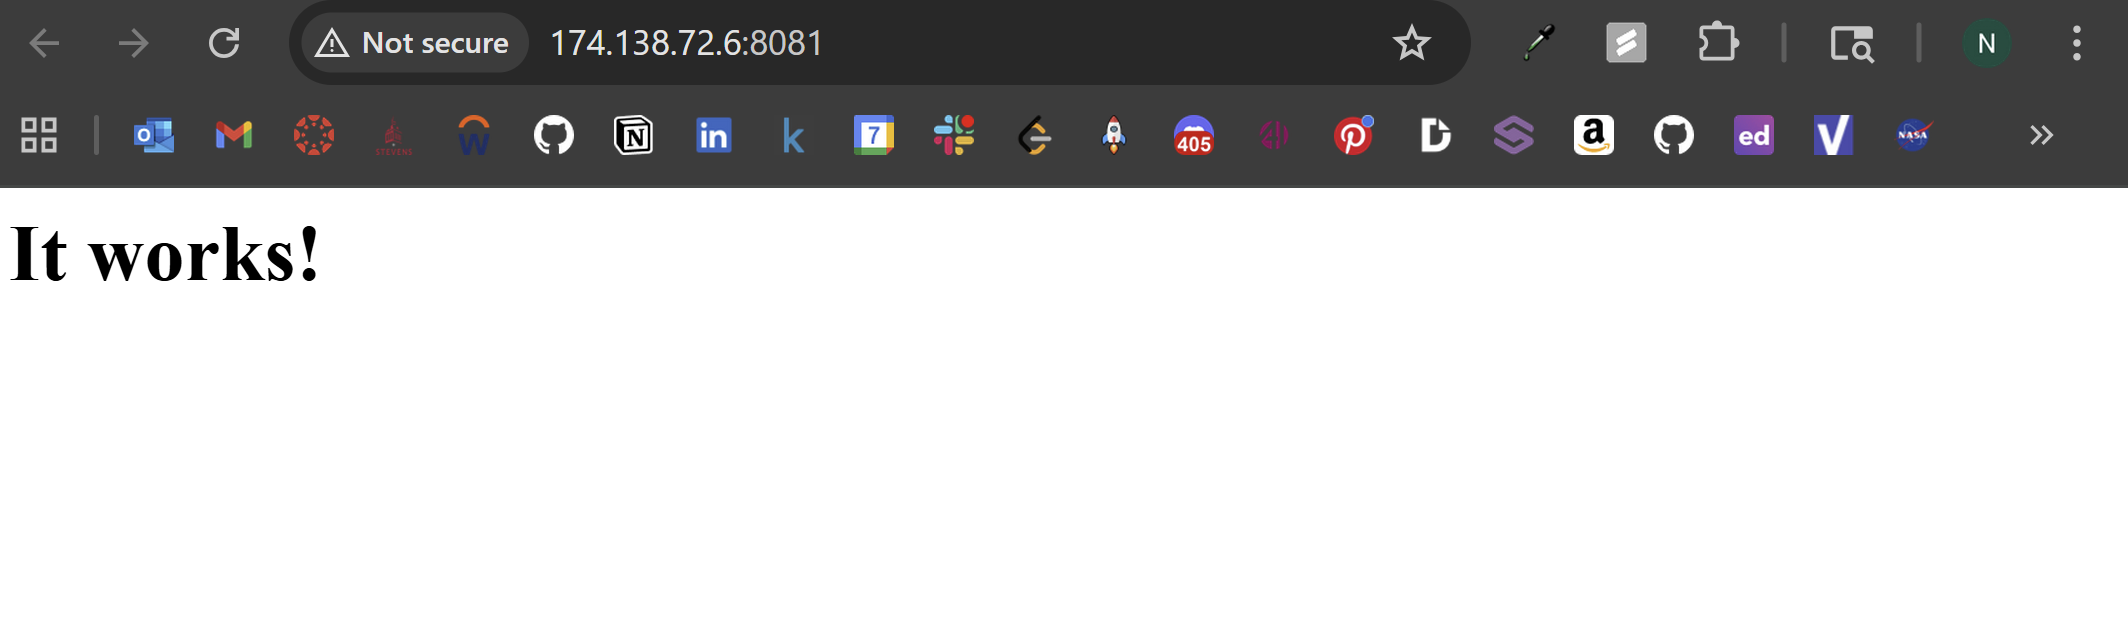
\includegraphics[width=0.6\linewidth]{Book_SSW590 (1)/eps/Screenshots/Overleaf_1.png}
    \caption{Working IP}
    \label{fig: Working IP}
\end{figure}


\begin{figure}[ht]
    \centering
    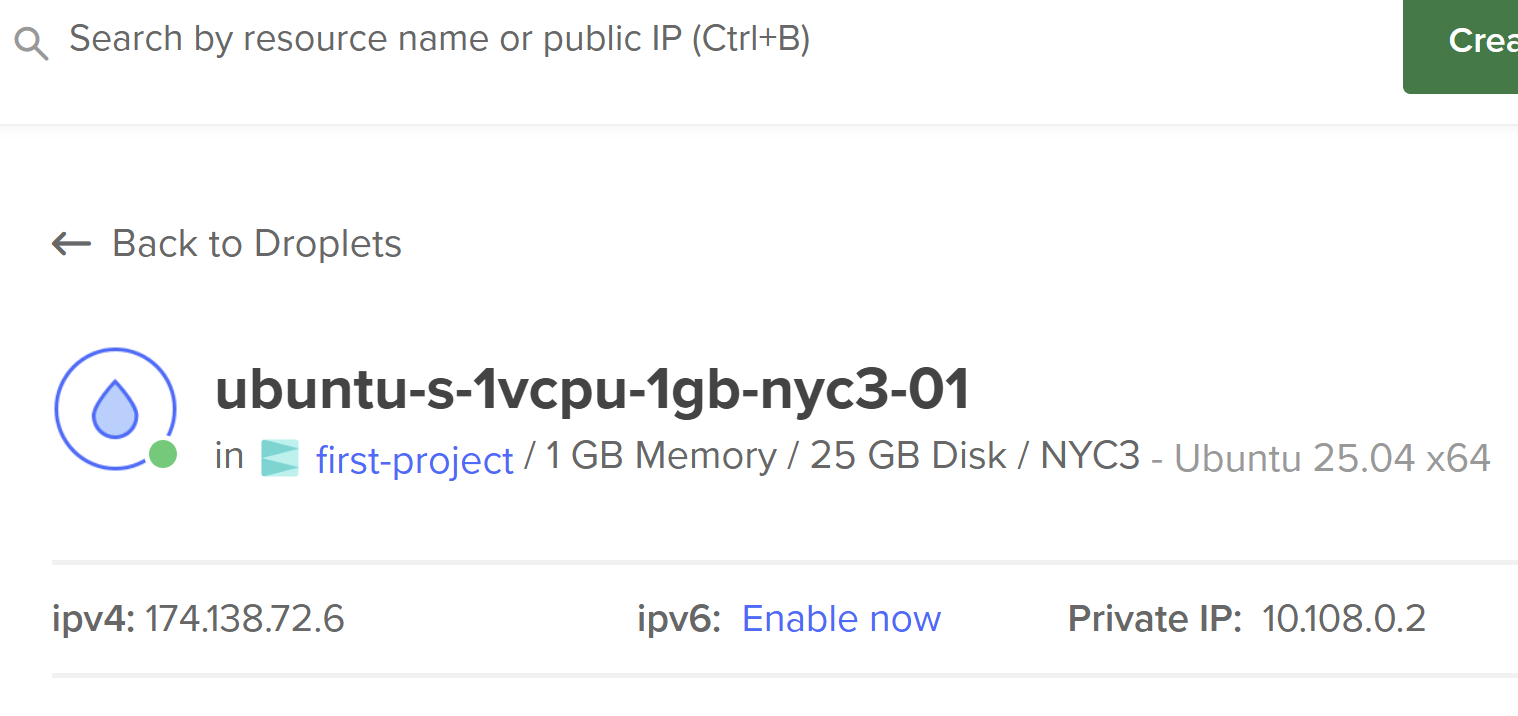
\includegraphics[width=0.6\linewidth]{Book_SSW590 (1)/eps/Screenshots/Overleaf_2.png}
    \caption{IP}
    \label{IP}
\end{figure}
